\section{El problema del viajante de comercio}

El problema del viajante de comercio consiste en hallar el recorrido con distancia
mínima en un conjunto de ciudades que pase por todas las ciudades y regrese al punto
inicial. \\

La implementación de los algoritmos es de la forma:
\begin{description}
 \item[Entrada:] Ficheros con ciudades indicadas como puntos en el plano según sus
 coordenadas.
 \item[Salida:] \texttt{vector<int>} con el orden en el que se recorren las ciudades.
\end{description}

En la salida nos ahorraremos repetir el primer nodo al final del recorrido.

Para todos los algoritmos utilizaremos una estructura de datos que nos permita manejar
el problema: la clase \texttt{Grafo} (en el fichero \texttt{grafo.h}). Un grafo consta
de:

\begin{itemize}
  \item Una \textbf{cantidad de nodos}, almacenada en el atributo \texttt{nodos}.
  \item Una \textbf{matriz de pesos}, almacenada en el vector \texttt{lados}.
\end{itemize}

La interfaz nos permite acceder y modificar estos datos con mayor facilidad.
Mediante los métodos \texttt{setPeso} y \texttt{peso} accederemos al peso de un
lado del grafo, y el método \texttt{pesosDesdeCoordenadas} nos permite inicializar el
grafo utilizando el formato de datos en el que aparece el problema: calculando
la distancia entre cualesquiera dos ciudades y añadir esta como peso de ese lado:

\lstinputlisting[firstline=47, lastline=51]{cpps/grafo.h}

Adicionalmente, la función \texttt{longitud} calcula la longitud de un camino dado,
teniendo en cuenta la distancia del último nodo al primero:

\lstinputlisting[firstline=54, lastline=59]{cpps/grafo.h}

Siendo \texttt{peso\_t} el tipo de dato con el que se manejen las distancias entre
nodos. Según el enunciado del problema (que pide que se redondee la distancia
euclídea al entero más próximo), será de tipo \texttt{int}.

\subsection{Algoritmos}

\subsubsection{Vecino más cercano}

Utilizando la estructura de datos explicada anteriormente, la resolución del problema
utilizando la heurística del vecino más cercano quedará:

\lstinputlisting[firstline=17, lastline=40]{cpps/tsp.cpp}

Tomamos como ciudad inicial el nodo 0 y almacenamos en la lista \texttt{disponibles}
las ciudades no visitadas. A continuación, mientras queden ciudades disponibles,
recorremos la lista buscando aquella ciudad con distancia mínima a la última, la
cual añadimos al trayecto y eliminamos de la lista de disponibles.

\subsubsection{Estrategias de inserción}

Para las estrategias de inserción realizamos el trabajo en 3 etapas.
En primer lugar hallamos las 3 ciudades que conforman el \textbf{recorrido inicial}.
Para ello basta tomar las ciudades como coordenadas en el plano y tomar las ciudades
más al norte, este y oeste (tomando los puntos con menor y mayor coordenada x y mayor
coordenada y):

\lstinputlisting[firstline=42, lastline=65]{cpps/tsp.cpp}

En el caso en el que el punto de mayor coordenada y sea también el de mayor (o menor)
coordenada x cogeremos el segundo con mayor (o menor) coordenada x.

Una vez conseguido un triángulo en el grafo lo suficientemente grande lo siguiente es añadir el resto de ciudades. Utilizaremos el siguiente procedmiento a la hora de insertar:

\begin{itemize}
  \item Recorrer la lista de nodos disponibles.
  \item Para cada nodo seleccionar el índice donde, de insertarse, aumente lo menos posible el peso del grafo.
  \item Insertamos en dicho índice el nodo que menos aumente el peso total.
\end{itemize}

\lstinputlisting[firstline = 85, lastline = 114]{cpps/tsp.cpp}
\newpage
El verdadero corazón del algoritmo reside en saber cómo varía el peso del grafo al insertar un nodo.
Consideremos lo siguiente: \\

Sea $y_0$ el nodo a insertar entre los nodos $n_i$ y $n_{i-1}$, que se encuentran seguidos, separados por un segmento $\overline{n_i \ n_{i-1}}$. Al hacer esta inserción el segmento que une los dos nuevos nodos deja de ser relevante en la longitud del recorrido y aparecen dos segmentos nuevos: $\overline{y_0 \ n_i}$ y $\overline{y_0 \ n_{i-1}}$.\\

Por tanto, el peso de la inserción de $n_0$ en el indice $i$ es:
$$ \operatorname{PesoInsercion}_i = \operatorname{Peso}(\overline{y_0 \ n_i})+\operatorname{Peso}(\overline{y_0 \ n_{i-1}})-\operatorname{Peso}(\overline{n_i \ n_{i-1}})$$

Primero buscamos cuál es el mínimo incremento de insertar el nodo $n_i$ y lo comparamos con los demás. Insertamos el nodo cuyo peso mínimo añadido sea menor en su índice correspondiente.

%% TODO: Explicación del resto de la estrategia

\subsubsection{Colonia de hormigas}

Como solución adicional propuesta por el equipo utilizamos una heurística basado en
colonias de hormigas. Este algoritmo se inspira en la comunicación por feromonas
de una colonia de hormigas para encontrar el camino óptimo hacia una fuente de comida. \\

Implementamos la Colonia (en el fichero \texttt{colonia.h}) mediante una clase. Una Colonia consta de:

\begin{itemize}
  \item Un grafo de \textbf{distancias} entre las ciudades.
  \item Un grafo con las \textbf{feromonas} de cada camino, inicialmente a un valor arbitrario.
  \item Una serie de constantes $\alpha, \beta, \rho, \xi, C, P, I$.
\end{itemize}

Las constantes controlan el comportamiento del algoritmo:

\begin{description}
  \item[$\alpha$] es el peso que tienen las feromonas a la hora de decantarse por un camino u otro.
  \item[$\beta$] es el peso que tienen la distancias en la circunstancia anterior.
  \item[$\rho$] es el coeficiente de evaporación de las feromonas.
  \item[$\xi$] es el coeficiente de debilitamiento de las feromonas.
  \item[$C$] determina cuánta feromona se añade a un camino.
  \item[$P$] es un flotante entre $0$ y $1$. Durante el progreso de un recorrido, hay
  una probabilidad de $1-P$ de que la hormiga opte por elegir el siguiente nodo de forma no aleatoria.
  \item[$I$] es la cantidad de feromona inicial en cada nodo.
\end{description}

Este algoritmo genera una serie de ciclos. En cada ciclo se empieza en un nodo al azar y se añaden nodos adicionales, formando un trayecto que termina cerrándose, decidiendo el siguiente nodo en función de la distancia al nodo actual y de la cantidad de feromona depositada en la arista entre ambos nodos.

Se define una fórmula que determina la probabilidad de escoger un nodo. Sea $i$ el nodo actual, $j$ un nodo candidato y $K$ la lista de nodos candidatos, la probabilidad de que se escoja el nodo $j$ a continuación del $i$ es:

$$P_{j}^i = \frac{(\tau_{i,j})^\alpha \cdot (1/d(i,j))^\beta}{\displaystyle \sum_{k \in K} (\tau_{i,k})^\alpha \cdot (1/d(i,k))^\beta}$$

Donde $\tau_{a,b}$ denota la cantidad de feromona depositada en la arista que une $a$ con $b$, y $d(a,b)$ es la distancia entre dos nodos $a$ y $b$. \\

En cada nodo, hay una probabilidad de $P$ de que se escoja un elemento a partir de la lista de probabilidades acumuladas (generando un flotante entre $0$ y $1$ y buscando la posición donde es superado), y una probabilidad de $1-P$ de que se tome directamente el elemento con mayor probabilidad de ser escogido. En la práctica no calcularemos el denominador de la expresión anterior y simplemente normalizaremos el flotante respecto del último elemento de la lista de probabilidades acumuladas. \\

Cada vez que una serie de hormigas termina su recorrido, se actualizan las feromonas de los nodos por los que han pasado. Para el mejor recorrido obtenido, la feromona de cada arista atravesada se multiplica por $1-\rho$ y se le suma $\rho C L^{-1}$, siendo $L^{-1}$ la inversa de la longitud del recorrido. En todos los recorridos, la feromona de cada arista recorrida se multiplica por $1-\xi$ y se le suma $\xi \cdot I$. Con esto se pretende potenciar el mejor recorrido y reducir el interés en las aristas que no han intervenido en ese camino, de forma que la próxima generación de hormigas optará por repetir caminos similares al óptimo evitando tomar aristas que no dieron resultado. \\

El algoritmo ejecuta varias generaciones de hormigas. Pueden usarse distintos criterios de parada, como por ejemplo detenerse cuando el mejor recorrido no se haya modificado en las últimas iteraciones, aunque optaremos por fijar el número de generaciones a un múltiplo del número de nodos del grafo.

\subsection{Comparativa de los algoritmos}

Para ver mejor las diferencias entre los tres algoritmos, hemos decidido ejecutarlos en algunos de los ejemplos propuestos, y hacer gráficos con los resultados. A continuación presentamos los caminos óptimos que deberían dar en cada uno de los ejemplos junto a lo que da cada algoritmo. Se adjunta, además, un diagrama de barras para poder apreciar mejor la eficacia de los resultados.

\subsubsection{Ejemplo 1: Ulysses16}


\begin{figure}[h]	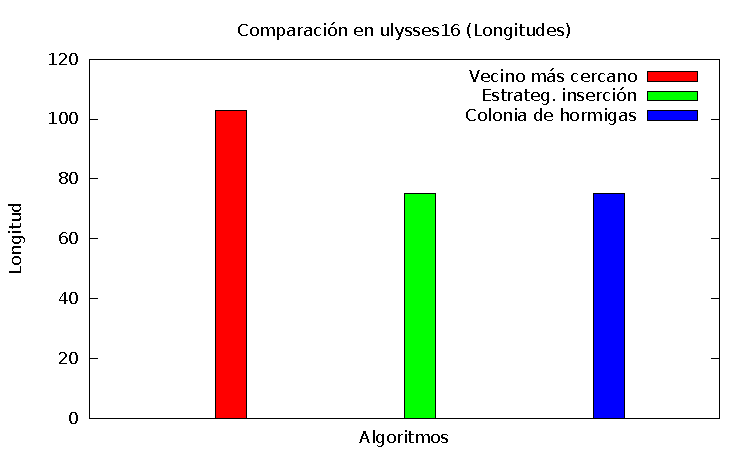
\includegraphics[width = 14cm ]{barras_ulysses16_longitud} \centering
	\caption{Comparativa de longitud de los caminos de cada algoritmo} \end{figure}


En el primer ejemplo tanto inserción como la colonia de hormigas dan un resultado muy bueno, mientras que el vecino más cercano se aleja bastante de estas distancias. Colocamos aquí los caminos realizados:

\begin{figure}[h]	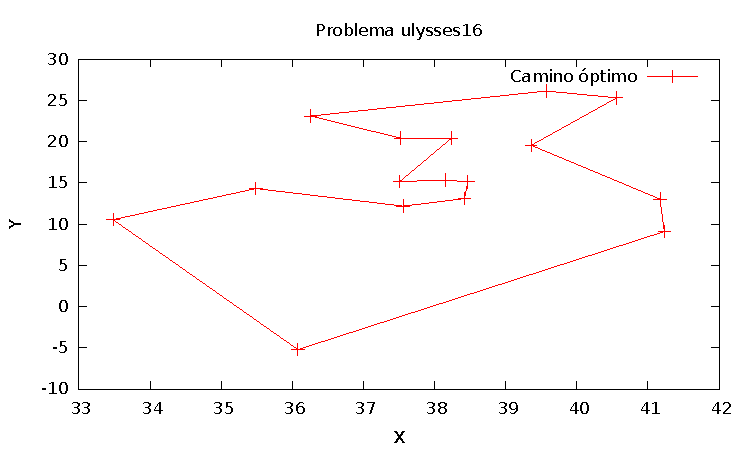
\includegraphics[width = \linewidth ]{ulysses16_tsp_opt} \centering
	\caption{Camino óptimo para el problema Ulysses16} \end{figure}

\begin{figure}[h]	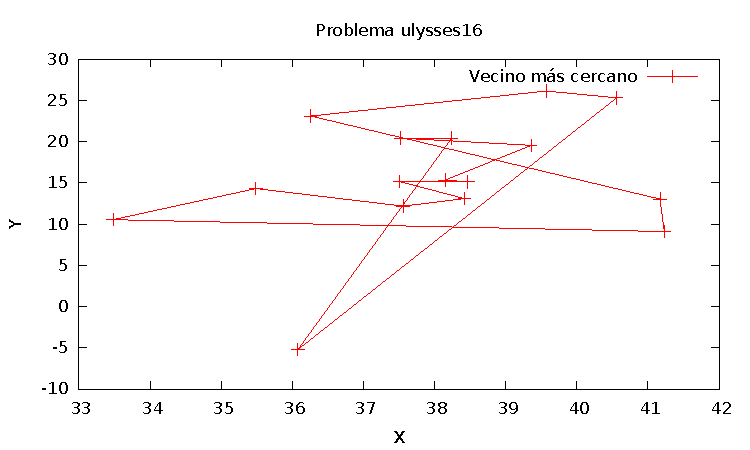
\includegraphics[width = \linewidth ]{ulysses16_tsp_1} \centering
	\caption{Camino proporcionado por el algoritmo del vecino más cercano} \end{figure}

\begin{figure}[h]	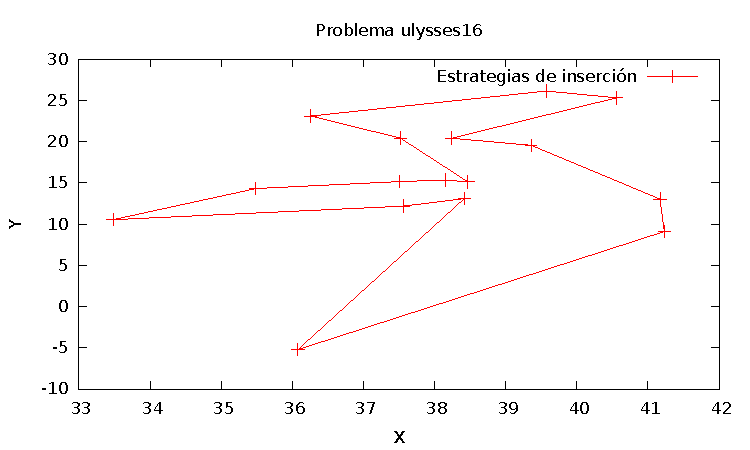
\includegraphics[width = \linewidth ]{ulysses16_tsp_2} \centering
	\caption{Camino proporcionado por el algoritmo de inserción} \end{figure}

\begin{figure}[h]	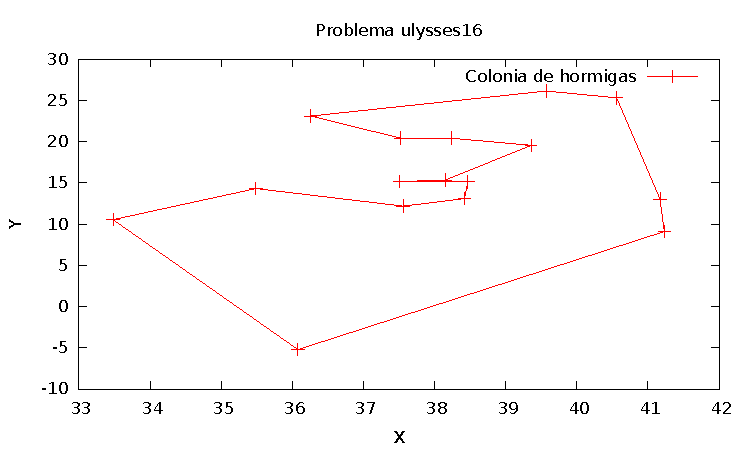
\includegraphics[width = \linewidth ]{ulysses16_tsp_3} \centering
	\caption{Camino proporcionado por el algoritmo de la colonia de hormigas} \end{figure}

\clearpage
\subsubsection{Ejemplo 2: Berlin52}


\begin{figure}[h]	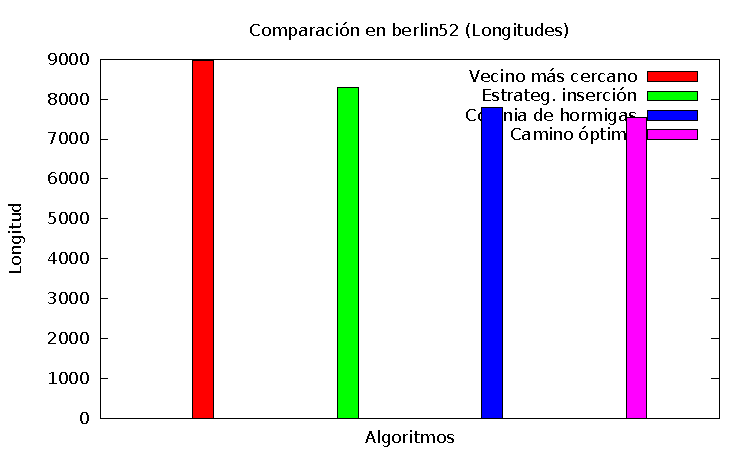
\includegraphics[width = 14cm]{barras_berlin52_longitud} \centering
	\caption{Comparativa de longitud de los caminos de cada algoritmo} \end{figure}


En este ejemplo el mejor resultado lo da el tercer algoritmo, la colonia de hormigas. A continuación se ponen los caminos realiados:

\begin{figure}[h]   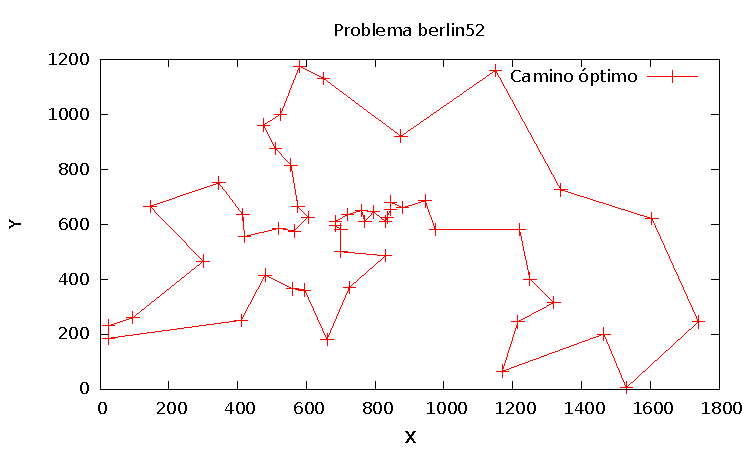
\includegraphics[width = \linewidth ]{berlin52_tsp_opt} \centering
	\caption{Camino óptimo para el problema Berlin52} \end{figure}

\begin{figure}	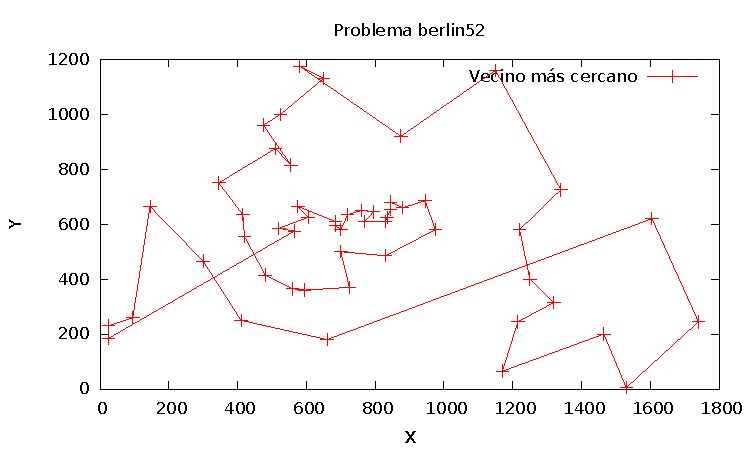
\includegraphics[width = \linewidth ]{berlin52_tsp_1} \centering
	\caption{Camino proporcionado por el algoritmo del vecino más cercano} \end{figure}

\begin{figure}	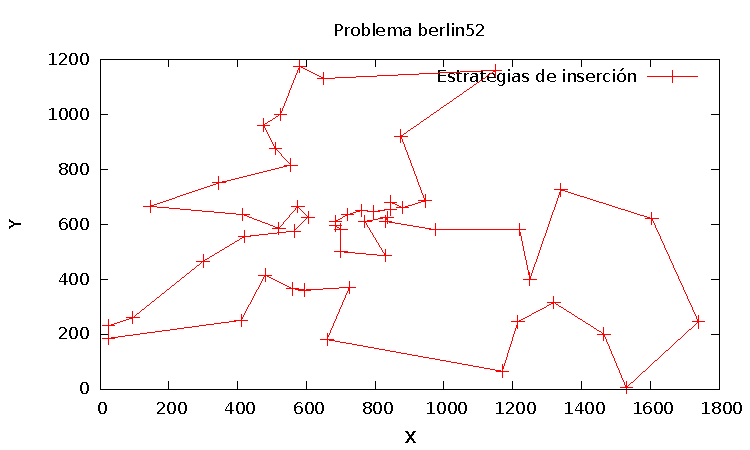
\includegraphics[width = \linewidth ]{berlin52_tsp_2} \centering
	\caption{Camino proporcionado por el algoritmo de inserción} \end{figure}

\begin{figure}	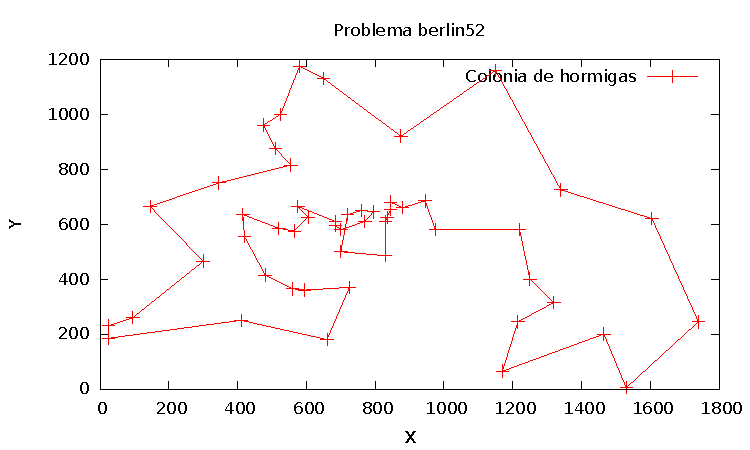
\includegraphics[width = \linewidth ]{berlin52_tsp_3} \centering
	\caption{Camino proporcionado por el algoritmo de la colonia de hormigas} \end{figure}

\clearpage
\subsubsection{Ejemplo 3: Pr76}

\begin{figure}[h]	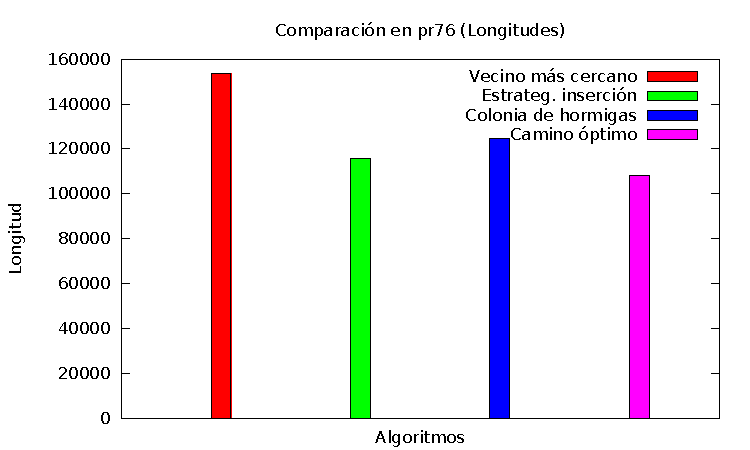
\includegraphics[width = 14cm ]{barras_pr76_longitud} \centering
	\caption{Comparativa de longitud de los caminos de cada algoritmo} \end{figure}

Por último, hemos colocado un ejemplo en el que el de inserción es el que mejor resultados da, ganando tanto a la colonia de hormigas como al vecino más cercano. Los caminos realizados son:

\begin{figure}	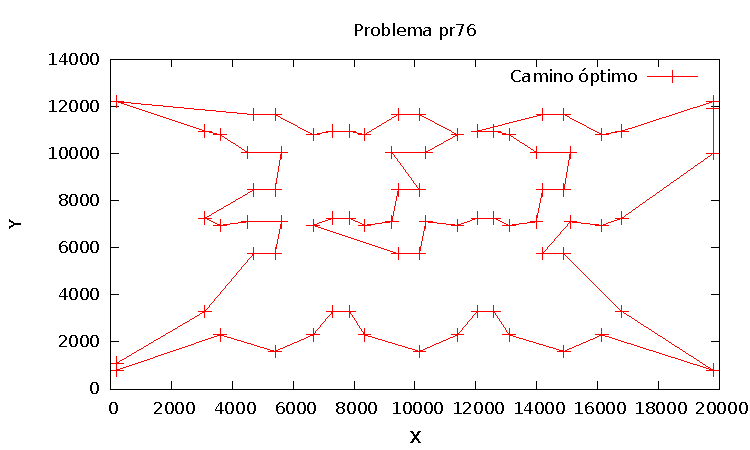
\includegraphics[width = \linewidth ]{pr76_tsp_opt} \centering
	\caption{Camino óptimo para el problema Pr76} \end{figure}

\begin{figure}	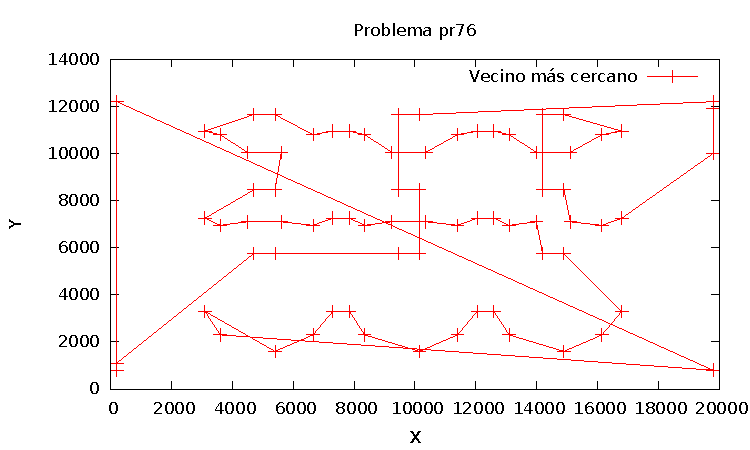
\includegraphics[width = \linewidth ]{pr76_tsp_1} \centering
	\caption{Camino proporcionado por el algoritmo del vecino más cercano} \end{figure}

\begin{figure}	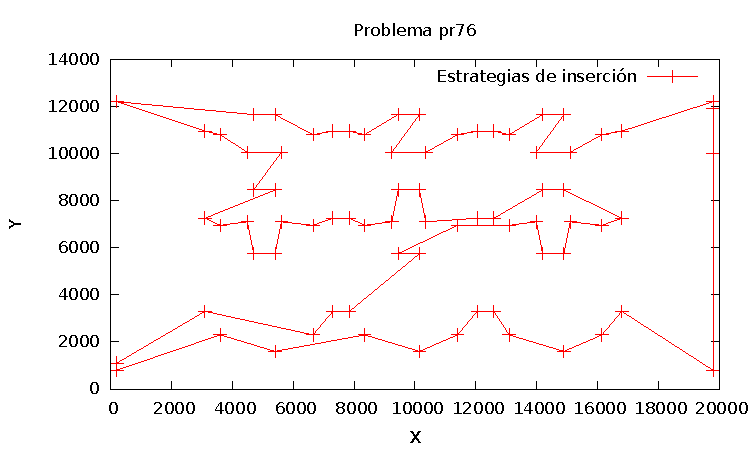
\includegraphics[width = \linewidth ]{pr76_tsp_2} \centering
	\caption{Camino proporcionado por el algoritmo de inserción} \end{figure}

\begin{figure}	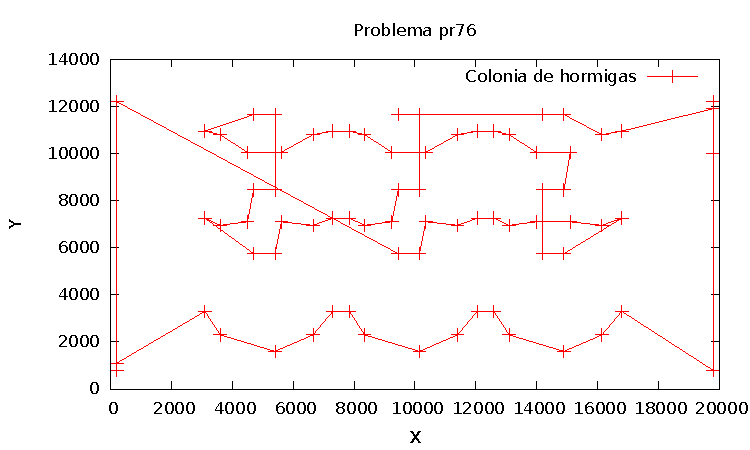
\includegraphics[width = \linewidth ]{pr76_tsp_3} \centering
	\caption{Camino proporcionado por el algoritmo de la colonia de hormigas} \end{figure}